
\documentclass[runningheads,a4paper]{llncs}

%\usepackage{amssymb}
%\setcounter{tocdepth}{3}
%\usepackage{graphicx}
%
%\usepackage{url}
%\urldef{\mailsa}\path|{alfred.hofmann, ursula.barth, ingrid.haas}@springer.com|
%\newcommand{\keywords}[1]{\par\addvspace\baselineskip
%\noindent\keywordname\enspace\ignorespaces#1}

%%%%%%%%%%%%%%%%%%%%%%%%%%%%%%%%%%%%%%%%%%%%%%%%%%%%%%%%%
%    Comments
%%%%%%%%%%%%%%%%%%%%%%%%%%%%%%%%%%%%%%%%%%%%%%%%%%%%%%%%%
\usepackage{blindtext}
\setcounter{tocdepth}{3}
\usepackage{verbatim}
\usepackage{framed}
%%%%%%%%%%%%%%%%%%%%%%%%%%%%%%%%%%%%%%%%%%%%%%%%%%%%%%%%%
%\usepackage[varg]{txfonts}
\usepackage{float}
\usepackage{wrapfig}
\usepackage{eqparbox}
\usepackage{booktabs}
\usepackage{stmaryrd}
\usepackage{amssymb}
\usepackage{mathrsfs}
\usepackage{epsfig,graphics}
\usepackage{amsmath}
\usepackage{wasysym}
\usepackage{graphicx}
\usepackage{tabularx}
\usepackage{url}
\usepackage{array}
%%%%%%%%%%%%%%%%%%%%%%%%%%%%%%%%%%%%%%%%%%%%%%%%%%%%%%%%%
%    Algorithm
%%%%%%%%%%%%%%%%%%%%%%%%%%%%%%%%%%%%%%%%%%%%%%%%%%%%%%%%%
\usepackage{multicol,pdflscape}
%\usepackage[]{algorithm2e}
\usepackage{algorithmicx}
\usepackage[linesnumbered,ruled]{algorithm2e}
\usepackage{algpseudocode}
%%%%%%%%%%%%%%%%%%%%%%%%%%%%%%%%%%%%%%%%%%%%%%%%%%%%%%%%%
%    Other Useful Packages
%%%%%%%%%%%%%%%%%%%%%%%%%%%%%%%%%%%%%%%%%%%%%%%%%%%%%%%%%
\usepackage{multirow}
\usepackage{extarrows}
\usepackage{xcolor}
\usepackage{listings}
\lstset{
    backgroundcolor=\color{white},
    basicstyle=\tt,
    keywordstyle=\color{blue},
    % add keywords
    morekeywords={IF, THEN, ELSE, END_IF},
    numbers=left,
%    numbersep=pt,
    numberstyle=\tiny\color{gray},
    title=\lstname,
    rulesepcolor=\color{red!20!green!20!blue!20},
    % set margin
    xleftmargin=2em,xrightmargin=2em, aboveskip=1em,
    % frame
    framexleftmargin=0.5mm,
    frame=shadowbox,
    % background color
    backgroundcolor=\color[RGB]{245,245,244},
    tabsize=4
}
%%%%%%%%%%%%%%%%%%%%%%%%%%%%%%%%%%%%%%%%%%%%%%%%%%%%%%%%%
\newcommand{\Real}{{\mathbb R}}
\newcommand{\Inh}[2]{\mathsf{Inh}\mathsf{(#1, #2)}}
\newcommand{\Cal}[2]{\mathsf{Cal}\mathsf{(#1, #2)}}
\newcommand{\Con}[2]{\mathsf{Con}\mathsf{(#1, #2)}}
\newcommand{\Cre}[2]{\mathsf{Cre}\mathsf{(#1, #2)}}
\newcommand{\Ref}[2]{\mathsf{Ref}\mathsf{(#1, #2)}}
\newcommand{\rand}{\wedge}
\newcommand{\ror}{\vee}
\newcommand{\rimply}{\Rightarrow}
\newcommand{\rr}{\rightarrow}
\newcommand{\nr}{\rightsquigarrow}
\newcommand{\rnot}{!}
\newcommand{\Instances}[1]{\mathsf{Inst}\mathsf{(#1)}}
\newcommand{\TypeOf}[1]{\mathsf{Type}\mathsf{(#1)}}
\newcommand{\AttrValue}[2]{\mathsf{AttrVal}\mathsf{(#1, #2)}}
\newcommand{\Value}[1]{\mathsf{Val}\mathsf{(#1)}}
\newcommand{\InitialValue}[1]{\mathsf{InitVal}\mathsf{(#1)}}
\newcommand{\Contains}[2]{\mathsf{Con}\mathsf{(#1, #2)}}
\newcommand{\patomic}{\mathsf{atomic}}
\newcommand{\pskip}{\mathsf{skip}}
\newcommand{\pmf}[1]{\mathsf{#1}}
\newcommand{\szihao}{\fontsize{1pt}{1pt}\selectfont}
\newcommand{\sfrac}{\szihao \dfrac}
\newcommand{\WI}[1]{{\itshape{\small{#1}}}}
\newcommand{\cname}[1]{{\small ${#1}$}}
\newcommand{\tabincell}[2]{\begin{tabular}{@{}#1@{}}#2\end{tabular}}
\renewcommand{\thefootnote}{\alph{footnote}}
% correct bad hyphenation here
\hyphenation{op-tical net-works semi-conduc-tor}
%\usepackage[square, comma, sort&compress, numbers]{natbib}
\usepackage{color}
\definecolor{gray}{rgb}{0.4,0.4,0.4}
\definecolor{darkblue}{rgb}{0.0,0.0,0.6}
\definecolor{cyan}{rgb}{0.0,0.6,0.6}
\usepackage{epstopdf}
\usepackage[colorlinks,
            linkcolor=black,
            anchorcolor=black,
            citecolor=blue,
			urlcolor=black,
            bookmarks=true
            ]{hyperref}
\newcommand{\TODO}[2]{{\textcolor{blue}{#1}}$\to${\textcolor{red}{#2}}}
\newcommand{\ASSIGN}[1]{{\textcolor{red}{#1}}}
\newcommand{\SOLVED}[2]{#2}
\newcommand{\keywords}[1]{\par\addvspace\baselineskip
\noindent\keywordname\enspace\ignorespaces#1}
\renewcommand\thesubsection{\Alph{subsection}}
%%%%%%%%%%%%%%%%%%%%%%%%%%%%%%%%%%%%%%%%%%%%%%%%%%%%%%%%%
%    Theorem Environment definition
%%%%%%%%%%%%%%%%%%%%%%%%%%%%%%%%%%%%%%%%%%%%%%%%%%%%%%%%%
\newtheorem{thm}{Theorem}
%\newtheorem{definition}{\bf Definition}



\begin{document}

\newcommand{\bahao}{\fontsize{8pt}{\baselineskip}\selectfont}
\newcommand{\badianwuhao}{\fontsize{8.5pt}{\baselineskip}\selectfont}
\newcommand{\jiuhao}{\fontsize{9pt}{\baselineskip}\selectfont}
\mainmatter  % start of an individual contribution

% first the title is needed
% \title{IMCL - An Event-Triggered Language for the Decomposition and Collaboration of Industrial System}
\title{Decomposition and Collaboration of Industrial Control System with Resource Constraints}

% a short form should be given in case it is too long for the running head
%\titlerunning{Lecture Notes in Computer Science: Authors' Instructions}
%\titlerunning{The Decomposition and Collaboration of Industrial System}
\titlerunning{Decomposition and Collaboration of Industrial Control System}



\author{
    \IEEEauthorblockN{Ju Li\IEEEauthorrefmark{2}, Jiawen Xiong\IEEEauthorrefmark{2},
    Xia Mao\IEEEauthorrefmark{2}, Jianqi Shi\IEEEauthorrefmark{2}, Xin Ye\IEEEauthorrefmark{3}, Yanhong Huang\IEEEauthorrefmark{2}\IEEEauthorrefmark{1}\thanks{$^{*}$Corresponding Author}
    }
    \IEEEauthorblockA{\IEEEauthorrefmark{2} National Trusted Embedded Software Engineering Technology Research Center\\
    East China Normal University, Shanghai, China\\
    %Email: \{jli, jwxiong, xmao, jqshi, yhhuang\} @sei.ecnu.edu.cn
    }
    \IEEEauthorblockA{\IEEEauthorrefmark{3} LIPN and Paris University 7, Paris, France \\
    Email: \{jli, jwxiong, xmao, jqshi, xye, yhhuang\}@sei.ecnu.edu.cn
    }
}


% author names and affiliations
% use a multiple column layout for up to three different
% affiliations
%\author{Haiping Pang$^\dag$, Ju Li$^\dag$, Yijia Ruan$^\dag$, Yanhong Huang$^{\ddag,*}$\thanks{$^{*}$Corresponding Author}, Jianqi Shi$^{\ddag}$ and Shengchao Qin$^\sharp$ \\
%$^\dag$Shanghai Key Laboratory of Trustworthy Computing, \\
%East China Normal University \\
%$^\ddag$National Trusted Embedded Software Engineering Technology Research Center,\\
%East China Normal University \\
%$^\sharp$  Teesside University \& Shenzhen University\\
%Email: \{hppang, jli, yjruan\}@ecnu.cn, \{yhhuang, jqshi\}@sei.ecnu.edu.cn, s.qin@tees.ac.uk
%}



\toctitle{Lecture Notes in Computer Science}
\tocauthor{Authors' Instructions}
\maketitle

\begin{abstract}
With the development of ``Industry 4.0'', the scale and complexity of industrial control system grow rapidly.
Hence, the analysis and verification of such systems face really big challenges.
Industry requires a reliable approach for decomposing the existing complex system model to multiple fine-grained and interactive models.
In this paper, we propose a general event-triggered language named \emph{IMCL} for modeling industrial control systems.
\emph{IMCL} can describe the physical resources and system in one unified model.
Specially, for the given resource constraints, we research the reliable and efficient approach of decomposition and collaboration based on \emph{IMCL} models to meet the industrial requirements. In particular, we have implemented the approach in our tool and get the encouraging results.

%With the \TODO{trend}{development} of ``Industry 4.0'', \TODO{the function and the intelligence of industrial system become sophisticated}{the scale and complexity of industrial system grows rapidly}.
%\TODO{Because there are more physical resources in the system, the industrial environment is more complicated.}{} Hence, the analysis and verification of such systems \TODO{have been much harder than before}{face really big challenges}.
%\TODO{It is a proper solution to decompose the complicated system model to multiple relatively simple models, and it is necessary to find a reliable way for the multiple models to collaborate with each other efficiently}{Industry requires a reliable approach for decomposing the existing complex system model to multiple fine-grained and interactive models.}.
%\TODO{In this paper, we introduce a general event-triggered language named \emph{IMCL} for modelling industrial systems.
%We show how \emph{IMCL} can describe the physical resources and system in one unified model.
%Within the given physical resource constraints, we present  reliable and efficient corresponding decomposition and collaboration algorithms based on \emph{IMCL} models. In particular, we have implemented these algorithms in a tool and get same satisfactory results.}{In this paper, we propose a general event-triggered language named \emph{IMCL} for modeling industrial systems.
%\emph{IMCL} describes the physical resources and system in one unified model.
%Following the given physical resource constraints, we present the reliable and efficient decomposition and collaboration algorithms based on \emph{IMCL} models to meet the industrial requirements. In particular, we have implemented these algorithms in a tool and get same encouraging results.}


%With the development of ``Industry 4.0'', the function and intelligence of industrial system become sophisticated.
%Because there are more physical resources in the system.
%The industrial environment is more complicated.
%Hence, the analysis and verification of such systems would be much harder than before.
%It is a proper solution to decompose the complicated system model to multiple Computing Units(CUs), and it is necessary to find a reliable way for the multiple CUs to collaborate with each other efficiently.
%In this paper, we propose a general event-triggered language named \emph{IMCL}, which can describe the physical resources and systems in one unified model.
%On the premise of the given physical resource constraints, we present the decomposition and collaboration algorithms that
%
%to ensure the consistency of the models during the
% that a collaborative multi-systems models can replace the complicated system model.
%On the premise of the given physical resource constraints, we propose the decomposition and collaboration algorithms based on the coordination of the system communication and collaboration functions. Ultimately, we can achieve the optimal solution that a collaborative multi-systems model can replace the traditional system model.


%\keywords{Program analysis, Industrial Control System, Model decomposition, Collaboration, Resource constraint}

\end{abstract}


% \keywords{Program analysis, Industrial Control System, Model decomposition, Collaboration, Resource constraint}


% It is a research focus to make use of the computing units(CUs) in the system, and it is a challenge to collaborate CUs with each other to partake the complicated system environment efficiently.

% ��һ�汾
% As the function and intelligence of industrial systems become more sophisticated, traditional single core processor will suffer more computing tasks. This paper aims to propose a method to decompose and collaborate one system under the physical resources constraint. Traditional single core processor is replaced by a cluster of heterogeneous and isomorphism computing units available in the system, enabling the replacement of a single model with multiple sub-models. In this paper, we propose a general event-triggered language named \emph{IMCL}, which can abstract the system resources and functions to achieve platform independence, and keeps the physical resources and systems in a unified model. On the premise of the given resource constraints, we propose the decomposition and collaboration algorithms based on the coordination of the system communication and collaboration functions, and ultimately to achieve the optimal solution that a collaborative multi-systems model can replace the traditional single-system model.

%\keywords{Program analysis, Model decomposition, Collaboration}
%\end{abstract}

% �ڶ��汾
%As the function and intelligence of industrial systems become sophisticated, the traditional industrial environment is becoming more complex and will suffer more computing tasks. It is a challenge to use multiple processors to collaborate with each other to partake the complex system environment efficiently. In this paper, we propose a method that the traditional processor can be replaced by a cluster of heterogeneous computing units available in one industrial system. To achieve platform independence of different systems, we present a general event-triggered language named \emph{IMCL}, which can describe the physical resources and systems in an unified model. On the premise of the given resource constraints, we propose the decomposition and collaboration algorithms based on the coordination of the system communication and collaboration functions, and ultimately to achieve the optimal solution that a collaborative multi-systems model can replace the traditional system model.


\section{Introduction}
``Industry 4.0" is a term originated by the German government for promoting the computerization of manufacturing\cite{industrial4}.
It involves the Cyber-Physical Systems (CPS), the Internet of Things (IoT) and cloudy computing etc in manufacturing. An industrial environment contains the normal work condition of people like offices, physical resources such as manufacturing equipment, storage and so on.
Many wireless networks monitor various aspects of the environment and transfer the data information to a central processor\cite{oliveira2011wireless}. Most of those actual industrial control systems are containing some Computing Units(CUs)\cite{GERO199065}. Every CU has the capability to process tasks and schedule specific physical resources.
However, there are many physical resources in a system. Meanwhile, the industrial control system has a variety of functions and is more intelligent. Hence, the traditional industrial environment has become more complex than before. It leads to the analysis and verification of such  systems more difficult. The cost of system research and application is more expensive.

% ����ϵͳ�����IJ���
To overcome the limitation, decomposition is used to reduce the complexity of the system for research and applications. \textbf{Decomposition} is a technique to master the function complexity of the model. Usually, a functional model can be replaced by a series of models of sub-systems after decomposition.
An actual industrial control system can be treated as a complex model. Every CU in a system can realize some part function of the system and can be considered as the corresponding models of sub-systems. Decomposition is a well-developed technique and it is widely applied to solve the problems brought by the function complexity.

However, most CUs have limits since the physical resource scheduling is limited.  If one system is too complex to be handled by one CU, it needs to use multiple CUs to collaborate with each other.
Many researchers \cite{DBLP:phd/de/Penzenstadler2010,henzinger2001giotto,damavandi2016modeling} have achieved great achievements about the collaboration of industrial system. Many researchers focus on the industrial intelligent ecosystem\cite{s16020215,deGeaFernandez2017} to handle the collection of massive data from the various devices dynamical collaboration.
But they didn't take the complex physical resources into consideration for the whole process of collaboration.
For example, there are three physical resources(\emph{res}1, \emph{res}2, \emph{res}3) in one system and all of those resources should work together, and two CUs($CU_{1}$, $CU_{2}$), where $CU_{1}$ is limited to schedule \emph{res}1 and \emph{res}2, and $CU_{2}$ is limited to schedule \emph{res}1 and \emph{res}3. Neither of the two CUs can implement the system. So, it is necessary to find the best solution to make the two CUs collaboration with each other to implement the system.

In our research, we introduce an event-triggered language called \emph{Industrial Modelling Collaboration Language}(\emph{IMCL}) which is platform-independent for heterogeneous systems. By this language, we can describe the physical resources and systems in one unified model.
Moreover, we propose the decomposition algorithms that can decompose the complicated system model to exact number of sub-systems appropriately corresponding to every CU with the constraints of resources. To maintain its functional consistency between sub-systems and original composited model, we present the collaboration algorithm. Besides, we show the evaluation method to get the optimizing solution of system collaboration.

The main contributions of this paper can be surmised as follows:
\begin{itemize}
  \item We propse an industrial model collaboration language, which can describe the system with complicated physical resources in a unified model.
  \item We provide the decomposition algorithm of the industrial model using \emph{IMCL}. This algorithm mainly includes the program analysis of control flow and data flow and the resource allocation with resource constraints.
  \item We implement the collaboration algorithm with the resource constraint based on the decomposed system. Moreover, we provide the evaluation way to get the most optimal solution for system collaboration.
\end{itemize}

% \subsection{Organization of this paper}

\medskip
\textbf{Outline}
\medskip

The remainder of this paper is organized as follows. In Section 2, we present the abstract of \emph{IMCL}. Section 3 proposes the approach for decomposition and collaboration. In Section 4, we introduce the decomposition algorithm. In Section 5, we discuss the collaboration algorithm. Section 6 shows the case study of one actual industrial control system.
%Section 7 introduces related works about our work. Section 8 closes the paper with a few concluding remarks.
Section 7 is the conclusion.

\medskip
\textbf{Related Work}
\medskip

The problem of the system decomposition and collaboration has much discussed in academic community during the past decades. The industry has been experimenting with different ways to develop new technologies to achieve better solutions for specific industrial environments\cite{korhonen2001four}.
% (Systems integration and collaboration in architecture, engineering, construction, and facilities management: A review)
In \cite{Shen2010196}, it presents that with the rapid advancement of information and communication technologies, particularly the Internet and Web-based technologies during the past years, various systems integration and collaboration technologies have been developed and deployed to different application domains, including architecture, engineering, construction, and facilities management.

% Using program synthesis for program analysis
Oxford University's latest research\cite{david2015using} proves that procedural decomposition and conversion is beneficial to procedural analysis.
% (Weiser,���Է���,���з���)
Weiser et al.\cite{weiser1981program} has proposed the program slicing method, which introduces how to slice a program with the data-flow and control-flow analysis. Jean Bertrand Gauthie\cite{DBLP:journals/orl/GauthierDL14} and Jingde Cheng\cite{Cheng:1993:SCP:646902.710201} have proved the decomposition theorems for linear programs and the approach of slicing concurrent programs, respectively.
The \cite{weiser1981program,DBLP:journals/orl/GauthierDL14,Cheng:1993:SCP:646902.710201} are influential on the basis principle of our decomposition algorithms.
% (Giotto)
Thomas A.Henzinger et al. present a time-triggered language \emph{Giotto}\cite{henzinger2001giotto}, which provides an abstract programmer's model for the implementation of one embedded control system with hard real-time constraints.
\emph{Giotto} can be annotated with platform constraints such as task-to-host mappings, and task and communication schedules. Different from \emph{Giotto}, our research focuses on the way how to describe the system with trigger events.
% (AutoBayes)
The NASA has released a toolkit \emph{AutoBayes}\cite{schumann2008autobayes} that can decompose and convert one system model from the perspective of the data analysis.
% (Better Requirements Decomposition Guidelines Can Improve Cost Estimation of Systems Engineering and Human Systems Integration)
Valerdi et al.\cite{valerdi2010better} details proposed updates to requirements decomposition guidelines that will help generate the number of system requirements.
% (A different view on system decomposition �C subsystem-centered property evaluation in multiple supersystems)
Arne Herberg et al.\cite{DBLP:conf/csdm/HerbergL13} motivates the need for enhanced support for subsystem development and evaluation in large engineering systems.
% (Decomposition of Systems and their Requirements -- Decomposition of Systems and their Requirements)
In \cite{DBLP:phd/de/Penzenstadler2010}, it introduces how to transition from one system to multi-subsystems using a criteria catalog and systematic requirement refinement, and we have inspired a lot from it. In our research, we mainly focus on the constraints of resources, which is the basis rule to decompose one IMCL system.
% (Industrial Internet of Things-Based Collaborative Sensing Intelligence: Framework and Research Challenges)
YuanFang Chen et al.\cite{s16020215} introduce the framework and research challenges about the industrial internet of things-Based collaborative sensing intelligence. Their paper thinks that an industrial intelligent ecosystem enables the collection of massive data from the various devices dynamically collaborating with humans. But in our work, we focus on the collaboration between computing units in the industrial control system.

% (Multi-Energy Industrial Systems[http://ecnu.summon.serialssolutions.com/#!/search?ho=t&l=zh-CN&q=Cooperation%20in%20Industrial%20Multi-agent%20Systems]��)
In \cite{Jennings91cooperationin,ferber1999multi,damavandi2016modeling,hanzo2009near}, plenty of researchers devote themselves to the research of multi-system and achieve great achievements.
% (Event-triggered distributed predictive control for the collaboration of multi-agent systems)
Zou et al.\cite{zou2016event} investigates  the problem of event-triggered distributed predictive control for multi-agent systems.
% (Consensus and Cooperation in Networked Multi-Agent Systems)
R.Olfati-Saber et al.\cite{4118472} provides a theoretical framework for the analysis of consensus algorithms for the decomposition of multi-agent networked system with an emphasis on the role if directed information flow, robustness to change in the network.
% (Decomposition Analysis of Indurstrial Power Demand of China based on Panel Data Model)
He et al.\cite{he2008decomposition} analyzes the decomposition under the industrial power demand.
% (iMRK: Demonstrator for Intelligent and Intuitive Human--Robot Collaboration in Industrial Manufacturing)
Dennis Mronga et al.\cite{deGeaFernandez2017} introduce the intelligent and intuitive dual-arm robotic system for industrial human-robot collaboration.
% (Developing collaboration mechanism for multi-agent systems with Petri net)
Fu-Shiung Hsieh \cite{DBLP:journals/eaai/Hsieh09} propose a collaboration mechanism of resource donation, including unilateral resource donation and reciprocal resource donation. During the process of our study, the collaboration algorithm basing on the premise of resource constraints. 



\section{Overall Approach}
This section presents our approach to realize the decomposition and collaboration for complex industrial control system. 
% Industrial Modelling Collaboration Language (IMCL)

\subsection{The Syntax of $IMCL$}
\emph{IMCL} is an event-triggered language. The event trigger is a system running mechanism that the processing of some function waiting for the event triggers and then execute the corresponding operation of this event. Here, we will introduce the abstract syntactic of \emph{IMCL}.
% ������ֵ
\begin{equation*}
    \begin{aligned}
        A_{exp} ::= &\ val \mid X \mid a_{0} + a_{1} \mid a_{0} - a_{1} \mid a_{0} * a_{1} \mid a_{0} / a_{1} \\
        B_{exp} ::= &\ \top \mid \bot \mid a_{0} = a_{1} \mid a_{0} \neq a_{1} \mid a_{0} > a_{1} \mid a_{0} < a_{1} \\
        C_{exp} ::= &\ channel!m \mid channel?m \mid sync.n \\
        E_{exp} ::= &\ E_{0};E_{1} \mid E_{0} \triangleleft b \triangleright E_{1} \mid b * E \mid X := a \mid C_{exp} \\
                    &\mid a \gg Dev \mid a \ll Dev \\
        T_{exp} ::= &\ trigger \ b \diamond E \mid trigger \ channel?m \diamond E  \\
    \end{aligned}
\end{equation*}

$A_{exp}$ is the arithmetic expression where $val$ is value, $X$ is variable, $a_{0}, a_{1} \in A_{exp}$.
$B_{exp}$ is the boolean expression, where $\top$ and $\bot$ are signifying the \emph{true} and \emph{false}. For every \emph{b} $\in$ $B_{exp}$, it is a bool expression. Next, we mainly introduce some specially expression in \emph{IMCL}. $C_{exp}$ is the communication expression. The $channel!m$ signifies sending a value $m$ from a $channel$ . The $channel?m$ signifies receiving a value $m$ from a $channel$. The $sync.n$ means to get the synchronous data $n$.
$E_{exp}$ is the execution expression. Condition choice $E_{0} \triangleleft b \triangleright E_{1}$ is that if $b$ is true then $E_{0}$, else $E_{1}$. The $b * E$ indicates that the $E$ will iterates until $b$ is false. Specifically, $a \gg Dev$ denotes that system transmit value $a$ to physical device $Dev$, while $Dev \ll a$ is getting $a$ from $Dev$. $T_{exp}$ is the event-triggered expression. The $trigger \ b \diamond E$ denotes an event $E$ happens when the $b$ is true. The $ trigger \ channel?m \diamond E_{exp}$ indicates that when receiving a $m$ from the $channel$, the event $E$ will begin to execute.

%\subsection{Modelling the Industrial System Using IMCL}
\subsection{\emph{IMCL} Model for Industrial Control System}

The modelling process focuses on system functions and features as following two steps:
\medskip
\textbf{Modelling the physical resources. }
Representations of physical resources are different based on diverse industrial environment, for instance, sensors, read-write devices, and the other resources. Considering their effects on the whole system, we describe all those resources as variables to unifying definition of resources.

\medskip
\textbf{Modelling the system. }
Observing its behavior, the nature of the system is gathering functions, read-write operations, and other actions together. Similar to physical resources, we model them as execution expressions. Multiple execution expressions in one specific order can make up one trigger event marked as $T$.

An \emph{IMCL} model consists of multiple concurrent trigger events, and every event is triggered only when its condition is satisfied. Let $\bowtie$ be the concurrent operation of two events such that $T_1\bowtie T_2$. Then, the \emph{IMCL} model \emph{Prog} can be defined:
\begin{displaymath}
Prog = \overset{n}{\underset{i=1}{\bowtie}} T_{i}, n \in N^{+}
\end{displaymath}


\section{Overall Approach}

This section presents our approach to realize the decomposition and collaboration for complex industrial control system.
% Industrial Modelling Collaboration Language (IMCL)

\subsection{The Syntax of $IMCL$}
\emph{IMCL} is an event-triggered language. The event trigger is a system running mechanism that the processing of some function waiting for the event triggers and then execute the corresponding operation of this event. Here, we will introduce the abstract syntactic of \emph{IMCL}.
% ������ֵ
\begin{equation*}
    \begin{aligned}
        A_{exp} ::= &\ val \mid X \mid a_{0} + a_{1} \mid a_{0} - a_{1} \mid a_{0} * a_{1} \mid a_{0} / a_{1} \\
        B_{exp} ::= &\ \top \mid \bot \mid a_{0} = a_{1} \mid a_{0} \neq a_{1} \mid a_{0} > a_{1} \mid a_{0} < a_{1} \\
        C_{exp} ::= &\ channel!m \mid channel?m \mid sync.n \\
        E_{exp} ::= &\ E_{0};E_{1} \mid E_{0} \triangleleft b \triangleright E_{1} \mid b * E \mid X := a \mid C_{exp} \\
                    &\mid a \gg Dev \mid a \ll Dev \\
        T_{exp} ::= &\ trigger \ b \diamond E \mid trigger \ channel?m \diamond E  \\
    \end{aligned}
\end{equation*}

$A_{exp}$ is the arithmetic expression where $val$ is value, $X$ is variable, $a_{0}, a_{1} \in A_{exp}$.
$B_{exp}$ is the boolean expression, where $\top$ and $\bot$ are signifying the \emph{true} and \emph{false}. For every \emph{b} $\in$ $B_{exp}$, it is a bool expression. Next, we mainly introduce some specially expression in \emph{IMCL}. $C_{exp}$ is the communication expression. The $channel!m$ signifies sending a value $m$ from a $channel$ . The $channel?m$ signifies receiving a value $m$ from a $channel$. The $sync.n$ means to get the synchronous data $n$.
$E_{exp}$ is the execution expression. Condition choice $E_{0} \triangleleft b \triangleright E_{1}$ is that if $b$ is true then $E_{0}$, else $E_{1}$. The $b * E$ indicates that the $E$ will iterates until $b$ is false. Specifically, $a \gg Dev$ denotes that system transmit value $a$ to physical device $Dev$, while $Dev \ll a$ is getting $a$ from $Dev$. $T_{exp}$ is the event-triggered expression. The $trigger \ b \diamond E$ denotes an event $E$ happens when the $b$ is true. The $ trigger \ channel?m \diamond E_{exp}$ indicates that when receiving a $m$ from the $channel$, the event $E$ will begin to execute.

%\subsection{Modelling the Industrial System Using IMCL}
\subsection{\emph{IMCL} Model for Industrial Control System}

The modeling process focuses on system functions and features as following two steps:

\textbf{Modeling the physical resources. }
Representations of physical resources are different based on diverse industrial environment, for instance, sensors, read-write devices, and the other resources. Considering their effects on the whole system, we describe all those resources as variables to unifying definition of resources.

\textbf{Modeling the system. }
Observing its behavior, the nature of the system is gathering functions, read-write operations, and other actions together. Similar to physical resources, we model them as execution expressions. Multiple execution expressions in one specific order can make up one trigger event marked as $T$.

An \emph{IMCL} model consists of multiple concurrent trigger events, and every event is triggered only when its condition is satisfied. Let $\bowtie$ be the concurrent operation of two events such that $T_1\bowtie T_2$. Then, the \emph{IMCL} model \emph{Prog} can be defined:
\begin{displaymath}
Prog = \overset{n}{\underset{i=1}{\bowtie}} T_{i}, n \in N^{+}
\end{displaymath}


For a given \emph{IMCL} program $Prog_{ori}$, we can get an AST(Abstract Syntax Tree) which contains details of its statements by an open source grammar parser tool, ANTLR.
Then, we can get the corresponding CFG(Control Flow Graph) and DFG(Data Flow Graph) based on AST.

A $CFG = \langle N, E \rangle$ is a directed graph, where \emph{N} is a set of nodes, and $E \subseteq N \times N$ is the set of edges while \emph{DFG} is a data-flow digraph structure. If $(n_1,n_2) \in E$, then $n_2$ is an immediate successor of $n_1$.

During the construction of CFG, we can get the information of each node. For each node $n$, we can have the following three sets: \emph{REF(n)}, \emph{DEF(n)} and \emph{INFL(n)}. \emph{REF(n)} is the set of variables whose values are used at n, and \emph{DEF(n)} is the set of variables whose values are changed at n. \emph{INFL(n)} is the set of nodes transitively control dependence on $n$, and it will not be empty only when $n$ has more than one immediate successor(for example, $n$ is a branch statement or a loop node).

There is a \emph{post} data-dependency($DD_{post}$) set of nodes for every node in the DFG, which is described as follow:\\
\begin{displaymath}
    \forall x \in DD_{post}(n), \ REF(x) \cap DEF(n) \neq \emptyset
\end{displaymath}
The $DD_{post}$(n) denotes that there are some nodes that are all data-depended on node $n$.
% For example, $DD_{post}(m) = \{2,6\}$, which means that at least one variable in both statement 2 and 6 are depended on statement $m$, respectively.

\textbf{SDG:} \ The \emph{System Dependence Graph}(SDG), a graph representation of system model with data dependence and control dependence, and which is based on \emph{CFG} and \emph{DFG}:
\begin{displaymath}
    SDG :=  \bigcup_{i=1}^{N} (CFG \oplus DD_{post}(i))
\end{displaymath}
which denotes that the SDG is a combination of CFG and all $DD_{post}$(i) that data-depended on every statement.

\begin{figure}[!ht]
    \centering
        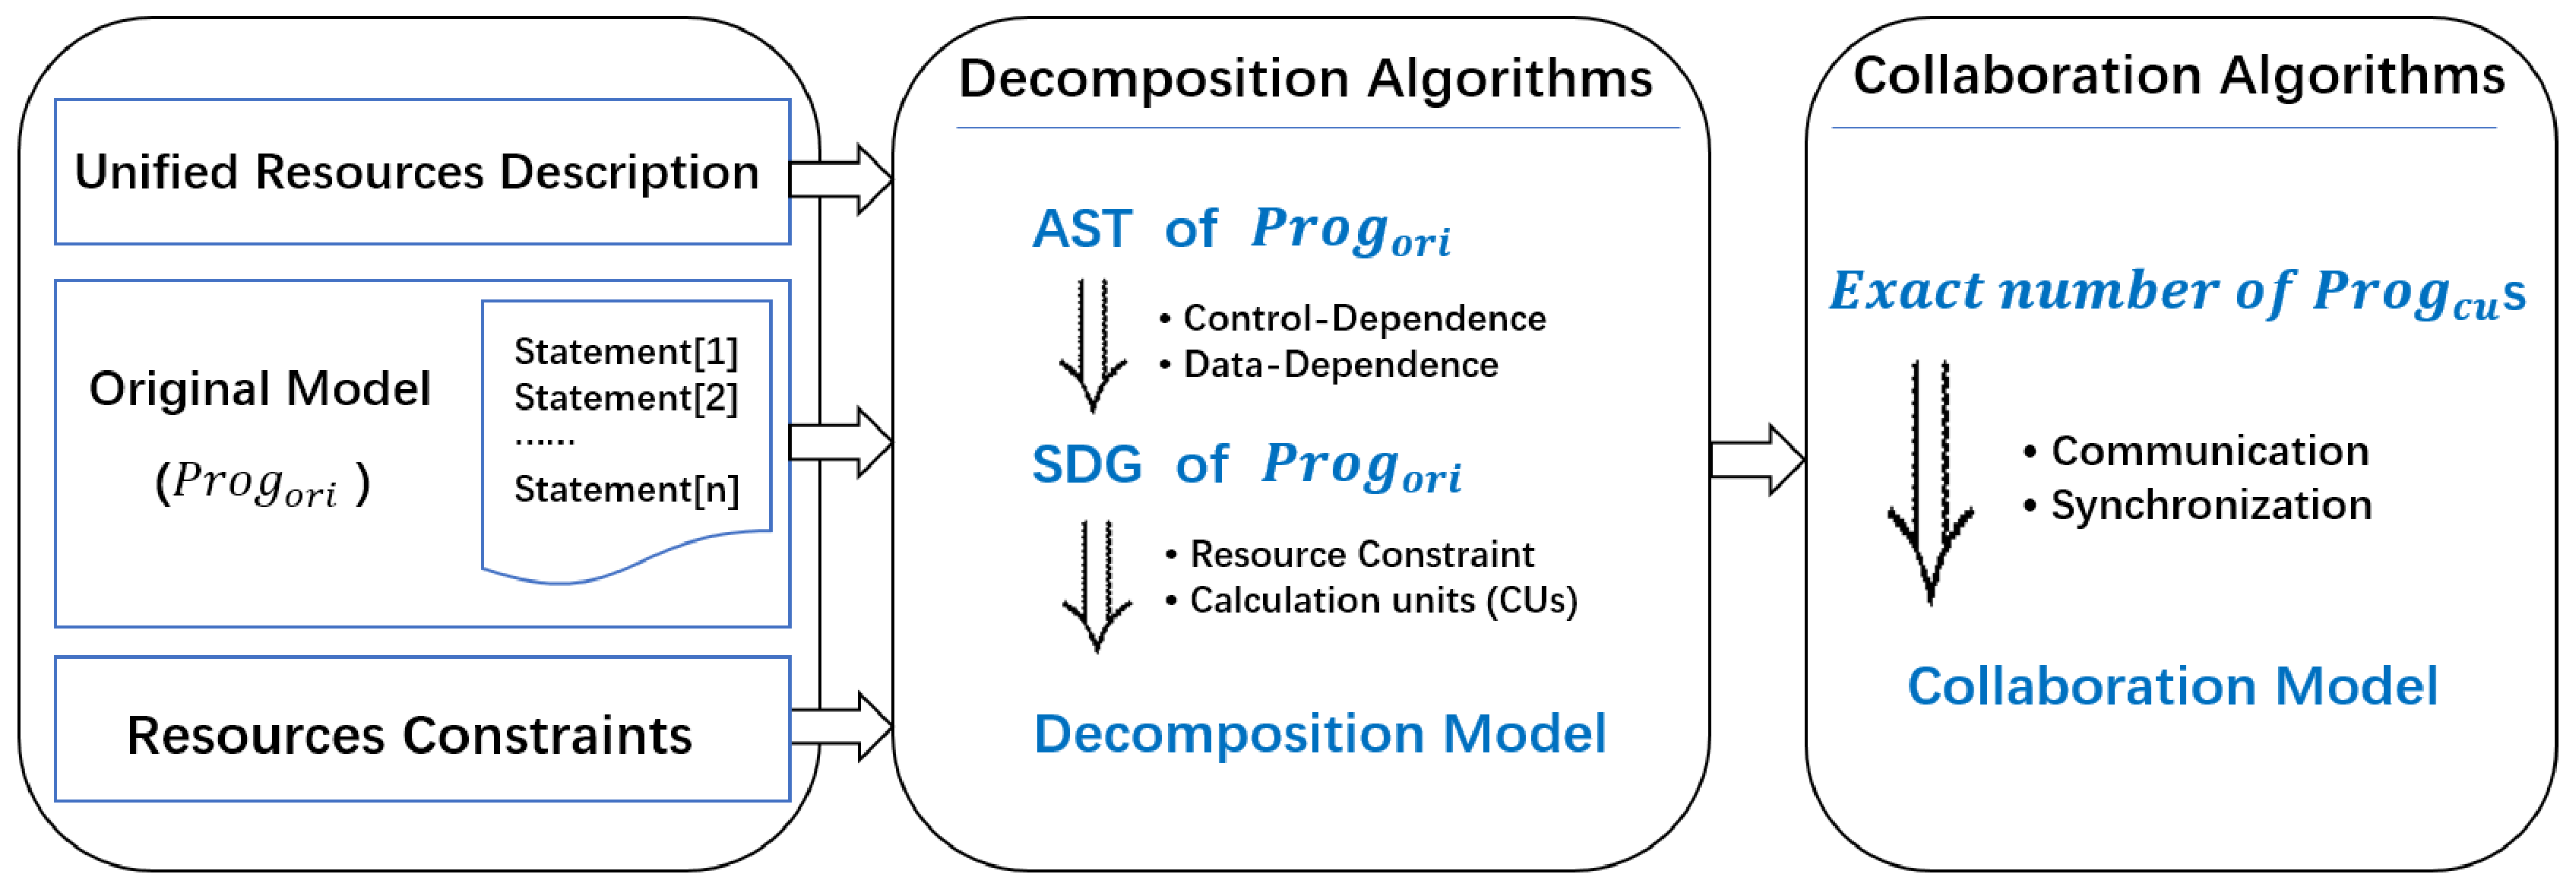
\includegraphics[height=1.5in, width=3.5in]{fig_Approach}
    \caption{Overview of approach for decomposition and collaboration }\label{fig_approach}
\end{figure}

Fig \ref{fig_approach} is the overview of the approach for decomposition and collaboration that we have implemented in our tool.
There are five basic terms for approach:
\begin{itemize}
  \item \textbf{Original Model:}\  The Original model is an \emph{IMCL} model $Prog_{ori}$ given at the beginning time, which is the description of an industrial control system.
  \item \textbf{Statement:}\ The $statement$ is the minimum computational task level for the program. Therefore, the $Prog_{ori}$ can be treated as a set of statements.
  \item \textbf{Resource Constraints:}\ It describes the constraints that physical resources are limited available for specific CUs.
  \item \textbf{Decomposition Model:}\  It is the multiple models that all of the statements in \emph{Original Model} are decompose to specified $CU$. In other words, it is transformed from a $Prog_{ori}$ with the resource constraint to the set of $Prog_{cu}$ for every \emph{CU}.
  \item \textbf{Collaboration Model:}\  Which is a set of the $Prog_{cu}$ interact with each other with communication and synchronization.
\end{itemize}

For one industrial control system, we model the physical resources and system as one \emph{Original Model} ($Prog_{ori}$) . Based on the SDG of $Prog_{ori}$, we can decompose the \emph{Original Model} to the \emph{Collaboration Model} with the resource constraints.
Only with the analysis of SDG, we can determinate the dependence of control flow and data flow to keep the constancy of \emph{Original Model} and \emph{Decomposition Model}.
%As a result, SDG analysis is a very important part of the decomposition.
To decompose the \emph{Original Model} into \emph{Decomposition Model} with resource constraints. $DD_{pre}$, the \emph{pre} data-dependency for each statement, can be obtained from corresponding $DD_{post}$. The definition is as follows:
\begin{displaymath}
    DD_{pre}(j) \ = \ \{ i \ | \ j \in DD_{post}(i), \ \forall i, j \in N \}
\end{displaymath}
where $j$ is a statement that data-depended on the statement in $DD_{pre}(j)$.
% For example, $DD_{pre}(j) = \{2, 7\}$ means that the statement $j$ are data-depended on statement $2$ and $7$.

The key to ensuring the reliability of \emph{Original Model} and \emph{Collaboration Model} is the communication in the process of collaboration, which is based on the SDG analysis.
We abstract the communication protocols between multiple models. The $IMCL$  unifies the communication and data synchronous among multiple models. There are three specific communication methods as follows:
\begin{itemize}
  \item \textbf{CHANNEL.CD!x} and \textbf{CHANNEL.CD?x},  the symbol \emph{CHANNEL.CD} is used for the control message and applied to the communication with control-dependence in multiple CUs or multiple internal event triggers in a signal CU. \emph{CHANNEL.CD!x} shows the model transmits a control message $x$ along the channel; \emph{CHANNEL.CD?x} denotes that receives the control message $x$ via the channel.
  \item \textbf{CHANNEL.DD!x:data} and \textbf{CHANNEL.DD?x:data},  \emph{CHANNEL.DD} is used for data message and is applied to the communication with data-dependence in multiple CUs or multiple internal triggers in a signal CU. \emph{CHANNEL.DD!x:data} shows the model transmits a data message $x$ with $data$ along the channel; \emph{CHANNEL.DD?x:data} denotes that a control message x with data via the channel.
  \item \textbf{SYNC.DATA:data},  the \emph{SYNC.DATA} is used to synchronize the data in different event triggers. Both \emph{CHANEL.DD} and \emph{SYNC.DATA} are used to synchronize the data. But different from \emph{CHANEL.DD}, \emph{SYNC.DATA} does no have any dependence on the $data$ in the original Model.
\end{itemize}

\section{Decomposition Algorithms}
Only with the analysis of SDG, we can determinate the dependence of control flow and data flow to keep the constancy of \emph{Original Model} and \emph{Decomposition Model}. As a result, SDG analysis is a very important part of the decomposition algorithms.

To decompose the \emph{Original Model} into \emph{Decomposition Model} with resource constraints. $DD_{pre}$, the \emph{pre} data-dependency for each statement, can be obtained from corresponding $DD_{post}$. The definition is as follows:
\begin{displaymath}
    DD_{pre}(j) \ = \ \{ i \ | \ j \in DD_{post}(i), \ \forall i, j \in N \}
\end{displaymath}
where $j$ is a statement that data-depended on the statement in $DD_{pre}(j)$.
% For example, $DD_{pre}(j) = \{2, 7\}$ means that the statement $j$ are data-depended on statement $2$ and $7$.

\section{Collaboration Algorithm}

The key to ensuring the reliability of \emph{Original Model} and \emph{Collaboration Model} is the communication in the process of collaboration, which is based on the SDG analysis.

We abstract the communication protocols between multiple models. The $IMCL$  unifies the communication and data synchronous among multiple models. There are three specific communication methods as follows:
\begin{itemize}
  \item \textbf{CHANNEL.CD!x} and \textbf{CHANNEL.CD?x},  the symbol \emph{CHANNEL.CD} is used for the control message and applied to the communication with control-dependence in multiple CUs or multiple internal event triggers in a signal CU. \emph{CHANNEL.CD!x} shows the model transmits a control message $x$ along the channel; \emph{CHANNEL.CD?x} denotes that receives the control message $x$ via the channel.
  \item \textbf{CHANNEL.DD!x:data} and \textbf{CHANNEL.DD?x:data},  \emph{CHANNEL.DD} is used for data message and is applied to the communication with data-dependence in multiple CUs or multiple internal triggers in a signal CU. \emph{CHANNEL.DD!x:data} shows the model transmits a data message $x$ with $data$ along the channel; \emph{CHANNEL.DD?x:data} denotes that a control message x with data via the channel.
  \item \textbf{SYNC.DATA:data},  the \emph{SYNC.DATA} is used to synchronize the data in different event triggers. Both \emph{CHANEL.DD} and \emph{SYNC.DATA} are used to synchronize the data. But different from \emph{CHANEL.DD}, \emph{SYNC.DATA} does no have any dependence on the $data$ in the original Model.
\end{itemize}


\section{Case Study}
An example of a real industrial \emph{product detection sorting system} will be shown to explain how the algorithms work.

\subsection{Product Detection Sorting System}
The product detection sorting system is mainly for product quality detecting, as well as sorting. The path delivery facility transmits the product to two conveyors by turns. Both the two conveyors have the \emph{read device} and \emph{write device}, respectively. The read device takes the info from the product to check the quality of the product, and then write the detecting results mark to the product. The sorting section separates the produce by scanning the detecting mark on the product and decide to sort the product into the qualified area or disqualified area.


\subsection{Implement of System Model}
As introduced above, we will describe how to model the system using $IMCL$. The implement of the system model includes three parts:

\textbf{(1) Unifying the resources.} \ \emph{SENSOR} and \emph{DEVICE} are the two types of resource sets where the system can get physical information. The system can get the info from these sensors and control those devices.

\begin{equation*}
\footnotesize
    \begin{aligned}
       & \textbf{SENSOR: }  \{ \ pathSensor, \ sensor1, \ sensor2, \ sortSensor \ \}; \\
       & \textbf{DEVICE: }  \{ \ \emph{PATHSET}, \ \emph{SREAD}1, \ \emph{SWRITE}1, \ \emph{SREAD}2, \ \emph{SWRITE}2, \\
       & \ \ \ \ \ \ \ \ \ \ \ \ \ \ \ \ \emph{SCANNER}, \ \emph{SORTSET} \ \};
    \end{aligned}
\end{equation*}

\begin{figure*}[!htb]
    \centering
        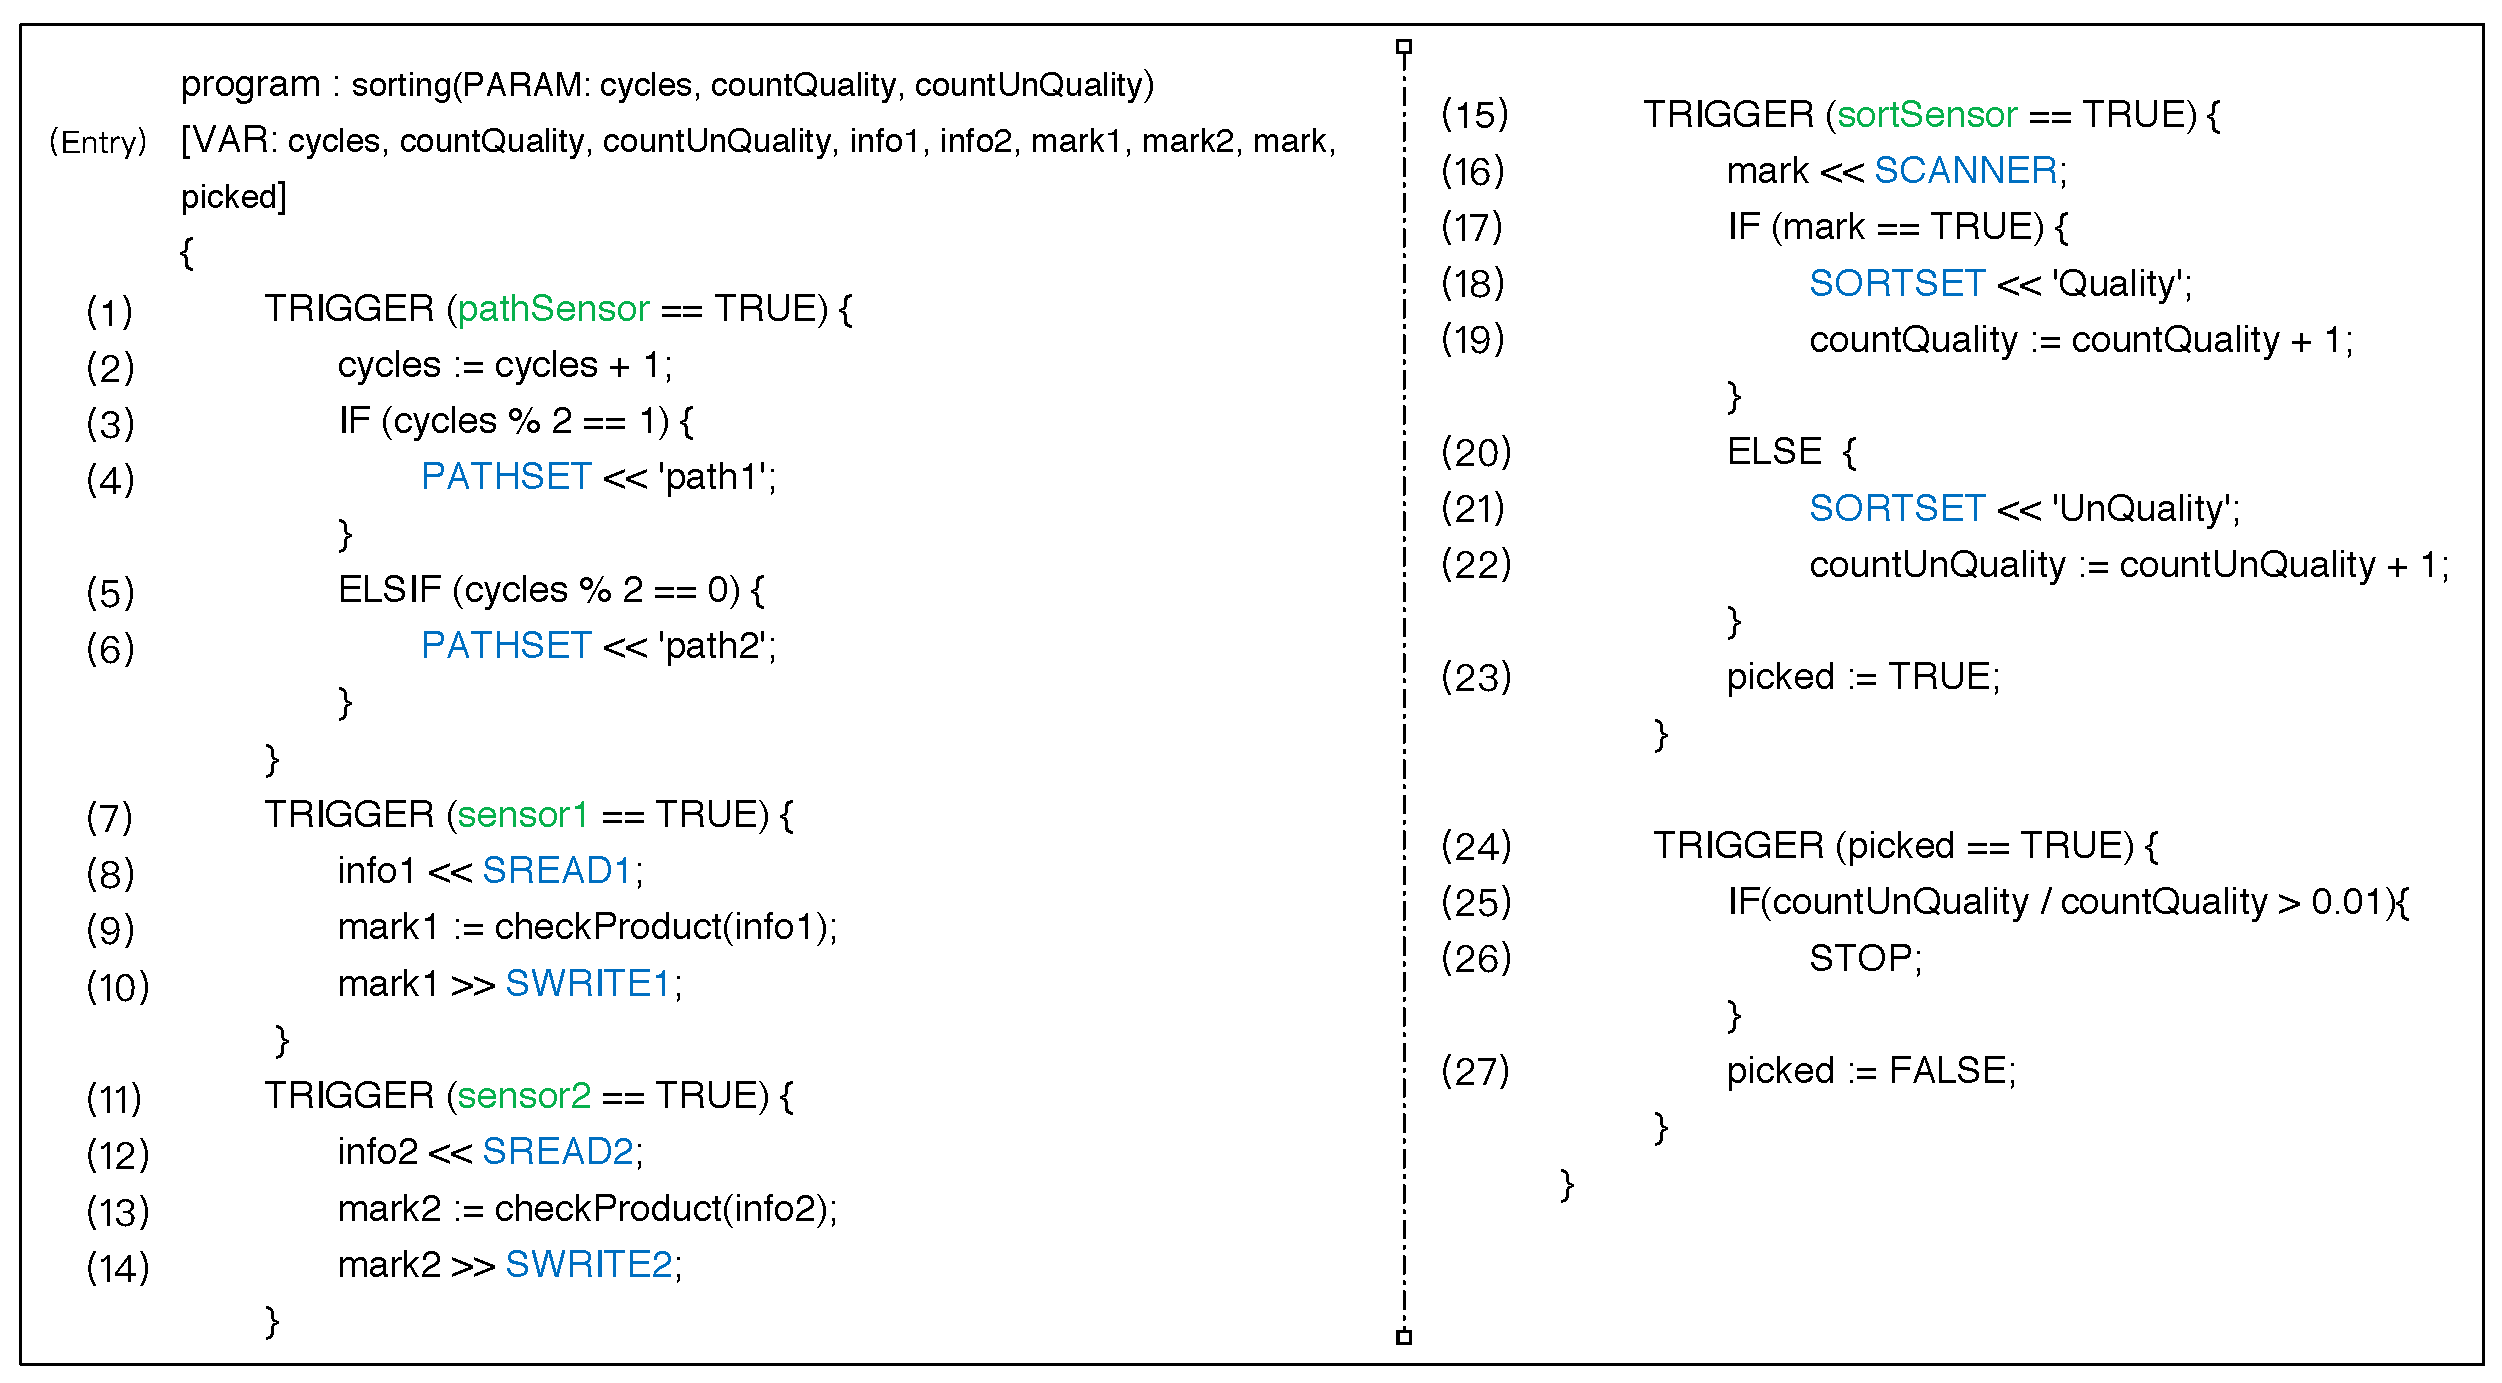
\includegraphics[height=3.0in, width=5.5in]{fig_IMCL_code}
    \caption{Modeling the system using IMCL}\label{fig_IMCL_code}
\end{figure*}

\textbf{(2) Modeling the system.} \ Fig.\ref{fig_IMCL_code} is the \emph{product detection sorting system}. The model contains five event triggers. The first one is triggered when \emph{pathSensor} is true, and \emph{PATHSET} will take a product to the two conveyors. The second one is triggered when the \emph{sensor1} is true; then the \emph{SEAD1} reads the information from the product to check whether it is qualified or not, and then the \emph{SWRITE1} marks the checking result on the product and so does the third event trigger. The fourth one indicates that when the \emph{pathSensor} is true, then the sorting device will determine the sorting of the product by the inspection mark on the product scanned by \emph{SCANNER}. The fifth one indicates that the system checks the system after the \emph{pick} becomes real.



\textbf{(3) Defining resource constraints.} \ The constraints of the resources describe the ability of every \emph{CU}. For example, the computing unit $B_{cu}$ can control two resources \emph{pathSensor} and \emph{PATHSET} in this system model.
\begin{equation*}
\footnotesize
    \begin{aligned}
        \ \textbf{constraint : \ } & \textbf{$A_{cu}$} \ \{ \ \emph{SCANNER}, \ sortSensor, \ \emph{SWRITE}1, \ \emph{SWRITE}2 \ \};\\
        \ \textbf{constraint : \ } & \textbf{$B_{cu}$} \ \{ \ pathSensor, \ \emph{PATHSET} \ \};\\
        \ \textbf{constraint : \ } & \textbf{$C_{cu}$} \ \{ \ sensor1, \ sensor2, \ \emph{SREAD}2, \ \emph{PATHSET} \ \};\\
        \ \textbf{constraint : \ } & \textbf{$D_{cu}$} \ \{ \ \emph{SREAD}1, \ \emph{SWRITE}1, \ \emph{SREAD}2, \ \emph{SORTSET} \ \};
    \end{aligned}
\end{equation*}

\subsection{Decomposition and Collaboration}
Base on the implementation of the model, collaboration model is obtained after decomposing the model with the resource constraints. The whole process consists the resource allocation, decomposition of the model and the collaboration with evaluation.

\textbf{(1) Resource allocation:} \
 \emph{SREAD}2, \emph{SWRITE}1, \emph{PATHSET} are all resource constraints that they can be used by more than one \emph{CU}, and eight solutions of resource constraints would be generated, and are listed in Table \ref{ResourcesAllocation}:

% begin{tabular}{|p{1cm}|p{2cm}|p{3cm}|}
\begin{table*}[!htb]
 \centering
% \tiny\tiny\scriptsize\footnotesize\small\normalsize\large\Large\LARGE\huge\Huge\footnotesize\small\normalsize\large\Large\LARGE\huge\Huge
%\bahao
\small
\caption{\label{ResourcesAllocation}Solutions that CUs are allocated with resources}
\begin{tabular}{|c|c|c|c|c|c|c|c|c|}

\hline

\multirow{2}{*}{\textbf{Resources}} &
\multicolumn{8}{|c|}{CUs allocated with resources ($CU_{\ast}$)} \\
\cline{2-9}
   &\textbf{ Sol 1 } &\textbf{ Sol 2 } &\textbf{ Sol 3 } &\textbf{ Sol 4 } &\textbf{Sol 5 } &\textbf{ Sol 6 } &\textbf{ Sol 7 } &\textbf{ Sol 8 }\\
\hline
\emph{sortSensor}   &$A_{cu}$ &$A_{cu}$ &$A_{cu}$ &$A_{cu}$ &$A_{cu}$ &$A_{cu}$ &$A_{cu}$ &$A_{cu}$ \\
\emph{sensor}2      &$C_{cu}$ &$C_{cu}$ &$C_{cu}$ &$C_{cu}$ &$C_{cu}$ &$C_{cu}$ &$C_{cu}$ &$C_{cu}$ \\
\emph{PATHSET}      &$B_{cu}$ &$C_{cu}$ &$B_{cu}$ &$C_{cu}$ &$B_{cu}$ &$C_{cu}$ &$B_{cu}$ &$C_{cu}$ \\
\emph{SWRITE}1      &$A_{cu}$ &$A_{cu}$ &$D_{cu}$ &$D_{cu}$ &$A_{cu}$ &$A_{cu}$ &$D_{cu}$ &$D_{cu}$ \\
\emph{SWRITE}2      &$A_{cu}$ &$A_{cu}$ &$A_{cu}$ &$A_{cu}$ &$A_{cu}$ &$A_{cu}$ &$A_{cu}$ &$A_{cu}$ \\
\emph{pathSensor}   &$B_{cu}$ &$B_{cu}$ &$B_{cu}$ &$B_{cu}$ &$B_{cu}$ &$B_{cu}$ &$B_{cu}$ &$B_{cu}$ \\
\emph{SORTSET}      &$D_{cu}$ &$D_{cu}$ &$D_{cu}$ &$D_{cu}$ &$D_{cu}$ &$D_{cu}$ &$D_{cu}$ &$D_{cu}$ \\
\emph{SCANNER}      &$A_{cu}$ &$A_{cu}$ &$A_{cu}$ &$A_{cu}$ &$A_{cu}$ &$A_{cu}$ &$A_{cu}$ &$A_{cu}$ \\
\emph{sensor}1      &$C_{cu}$ &$C_{cu}$ &$C_{cu}$ &$C_{cu}$ &$C_{cu}$ &$C_{cu}$ &$C_{cu}$ &$C_{cu}$ \\
\emph{SREAD}1       &$D_{cu}$ &$D_{cu}$ &$D_{cu}$ &$D_{cu}$ &$D_{cu}$ &$D_{cu}$ &$D_{cu}$ &$D_{cu}$ \\
\emph{SREAD}2       &$C_{cu}$ &$C_{cu}$ &$C_{cu}$ &$C_{cu}$ &$D_{cu}$ &$D_{cu}$ &$D_{cu}$ &$D_{cu}$ \\

\hline
\end{tabular}
\end{table*}


% 介绍了不同solution下的不同的分解结果
\textbf{(2) Optimization of Decomposition and Collaboration:} \
There are eight results shown in Table \ref{Evaluations} corresponding to the eight solutions in Table \ref{ResourcesAllocation}.

%\begin{table}[htbp]
\begin{table*}[!htb]
\centering
% \tiny\tiny\scriptsize\footnotesize\small\normalsize\large\Large\LARGE\huge\Huge\footnotesize\small\normalsize\large\Large\LARGE\huge\Huge
\small
\caption{\label{Evaluations}The results of our algorithms for different evaluations}
\begin{tabular}{|c|c|c|c|c|c|c|c|c|}
\hline
\multirow{2}{*}{} &
\multicolumn{4}{|c|}{\textbf{Decompositions}} & \multicolumn{3}{|c|}{\textbf{Collaborations}} &
\multirow{2}{*}{\textbf{Evals}} \\
\cline{2-8}
   &$A_{cu}$ &$B_{cu}$ &$C_{cu}$ &$D_{cu}$ &\emph{ CD } &\emph{ DD } &\emph{SYNC} \\

\hline
\textbf{Sol 1}    &\tabincell{c}{\{ 9,10,13,14,15,16,\\17,19,20,22,23 \}} &\tabincell{c}{\{1,2,3,4,5,6,\\24,25,26,27\}} &\tabincell{c}{\{7,11,12\}} &\tabincell{c}{\{8,18,21\}} &7 &2 &3 &$1.833$ \\
% 0.3*8*8 + 0.4*5*5 + 0.5*1*1 = 29.7
\hline
\textbf{Sol 2}    &\tabincell{c}{\{ 9,10,13,14,15,16,\\17,19,20,22,23 \}} &\tabincell{c}{\{1,2,3,5,24,\\25,26,27\}} &\tabincell{c}{\{4,6,7,\\11,12\}} &\tabincell{c}{\{8,18,21\}} &11 &2 &2 &$2.167$ \\
% 0.3*12*12 + 0.4*5*5 + 0.5*1*1 = 53.7
\hline
\textbf{Sol 3}    &\tabincell{c}{\{ 13,14,15,16,17,\\19,20,22,23 \}} &\tabincell{c}{\{1,2,3,4,5,6,\\24,25,26,27\}} &\tabincell{c}{\{7,11,12\}} &\tabincell{c}{\{8,9,10,\\18,21\}} &\textbf{6} &\textbf{1} &\textbf{2} &\textbf{0.333} \\
% 0.3*7*7 + 0.4*4*4 + 0.5*1*1 = 21.6
\hline
\textbf{Sol 4}    &\tabincell{c}{\{ 13,14,15,16,\\17,19,20,22,23 \}} &\tabincell{c}{\{1,2,3,5,24,\\25,26,27\}} &\tabincell{c}{\{4,6,7,\\11,12\}} &\tabincell{c}{\{8,9,10,\\18,21\}} &10 &1 &2 &$1.0$ \\
% 0.3*11*11 + 0.4*4*4 + 0.5*1*1 = 43.2
\hline
\textbf{Sol 5}    &\tabincell{c}{\{ 1,2,3,4,5,6,\\24,25,26,27 \}} &\tabincell{c}{\{1,2,3,4,5,6,\\24,25,26,27\}} &\tabincell{c}{\{7,11\}} &\tabincell{c}{\{8,12,18,21\}} &8 &2 &2 &$1.667$ \\
% 0.3*8*8 + 0.4*4*4 + 0.5*1*1 = 26.1
\hline
\textbf{Sol 6}    &\tabincell{c}{\{ 9,10,13,14,15,16,\\17,19,20,22,23\}} &\tabincell{c}{\{1,2,3,5,24,\\25,26,27\}} &\tabincell{c}{\{4,6,7,11\}} &\tabincell{c}{\{8,12,18,21\}} &12 &2 &1 &$2.0$ \\
% 0.3*12*12 + 0.4*4*4 + 0.5*1*1 = 50.1
\hline
\textbf{Sol 7}    &\tabincell{c}{\{ 13,14,15,16,17,\\19,20,22,23 \}} &\tabincell{c}{\{1,2,3,4,5,6,\\24,25,26,27\}} &\tabincell{c}{\{7,11\}} &\tabincell{c}{\{8,9,10,\\12,18,21\}} &7 &1 &2 &$1.167$ \\
% 0.3*7*7 + 0.4*3*3 + 0.5*1*1 = 18.8
\hline
\textbf{Sol 8 }    &\tabincell{c}{\{13,14,15,16,17,\\19,20,22,23 \}} &\tabincell{c}{\{1,2,3,5,24,\\25,26,27\}} &\tabincell{c}{\{4,6,7,11\}} &\tabincell{c}{\{8,9,10,\\12,18,21\}} &11 &1 &3 &$1.5$ \\
% 0.3*11*11 + 0.4*3*3 + 0.5*1*1 = 40.4
\hline
\end{tabular}
\end{table*}

\begin{figure*}[!htb]
    \centering
        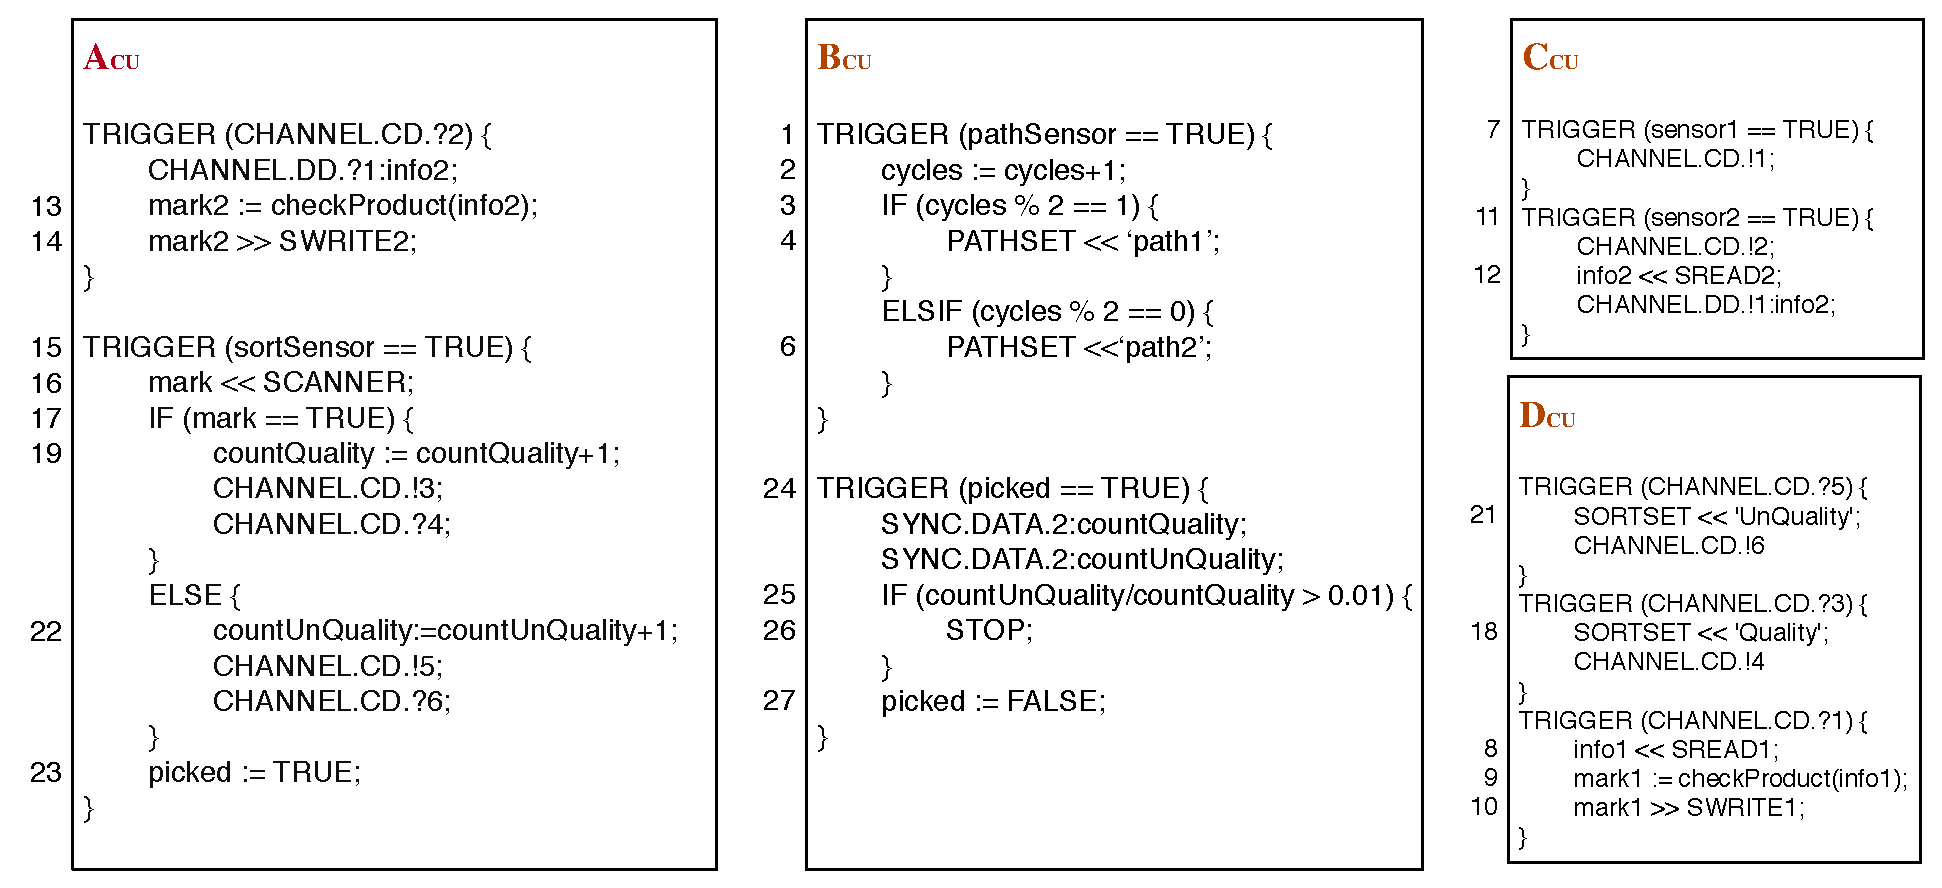
\includegraphics[height=2.7in, width=6.0in]{fig_four_collaborated_program}
    \caption{The collaboration of $A_{cu}$, $B_{cu}$, $C_{cu}$ and $D_{cu}$}\label{fig_four_collaborated_program}
\end{figure*}

As shown in Fig.\ref{fig_IMCL_code}, there are 27 statements in the model that every statement is the minimum computational task level we want to decompose. Table \ref{ResourcesAllocation} shows the eight solutions decomposing the model. In every solution, each \emph{CU} has a set of statements, which means that the \emph{CU} can take the minimum computational tasks in the original model. For example, in \emph{Sol 1}, the $C_{cu}$ decomposed with the set $\{7,11,12\}$, meaning that the $C_{cu}$ are labeled to statement 7, 11 and 12 in sorting system model. The \emph{Collaborations} in this table has three sub-parts: the \emph{CD} shows the number of control dependencies in the collaborative system; the \emph{DD} represents the number of data dependence in the collaborative system; the \emph{SYNC} is the number of data synchronization in the collaborative system. The \emph{Evals} is the evaluation of the collaboration for every solution, and it is the valuation standard of various solutions.
% We set the value \mathrm{}of $w_{cd}$, $w_{dd}$ and $w_{sync}$ in evaluation $Eval$ are $0.3$, $0.4$ and $0.5$ respectively(of course, researcher or developer can assign the value by their actual need).

From the results in Table \ref{Evaluations}, we can conclude that the \emph{Sol} 3 is the most optimizing solution to decompose and collaborate the model. The collaboration of four CUs are shown in Fig.\ref{fig_four_collaborated_program}.

The implementation of this case study can be cloned from our git repository\footnote{http://code.ntesec.com.cn/ju.li/model-slicing.git}.


%\begin{table}[htbp]
%\centering
%\caption{\label{comparison}Result comparison on LN data}
%\begin{tabular}{c|c|c|c|c|c|c|c}
%\hline
%\multirow{2}{*}{Instance} &
%\multirow{2}{*}{Original Instance} &
%\multirow{2}{*}{High Priority} &
%\multirow{2}{*}{Low Priority} &.
%
%\multicolumn{2}{|c|}{Benchmark} & \multicolumn{2}{|c}{Our Algorithm} \\
%\cline{5-8}
%& & & & Utilization & Time(s) & Utilization & Time(s)\\
%\hline
%LN01\&02  &  LN01 \& LN02    &     LN01      &    LN02     &  99.3\%   & 624 &    &   \\
%
%\hline
%\end{tabular}
%\end{table}
%



%\begin{table}[htbp]
%\centering
%\caption{\label{ResourcesAllocation}Result comparison on LN data}
%\begin{tabular}{|c|c|c|c|c|c|c|c|c|c|c|c|}
%\hline
%\scriptsize
%\multirow{2}{*}{Solution} &
%
%
%\multicolumn{11}{|c|}{CUs allocatedwith resources} \\
%\cline{2-12}
%   &\tabincell{c}{path-\\Sensor} &sensor1 &sensor2 &sortSensor &PATHSET &SREAD1 &SWRITE1 &SREAD2 &SWRITE2 &SCANNER &SORTSET \\
%
%\hline
%s0 &s1 &s2 &s3 &s4 &$\backslash$ &r6 &s7 &s8 &r9 &s10 &s11 \\
%s0 &s1 &s2 &s3 &s4 &s5 &r6 &s7 &s8 &r9 &s10 &s11 \\
%s0 &s1 &s2 &s3 &s4 &s5 &r6 &s7 &s8 &r9 &s10 &s11 \\
%
%\hline
%\end{tabular}
%\end{table}


% \section{Related Work}

The problem of the system decomposition and collaboration has much discussed in academic community during the past decades. The industry has been experimenting with different ways to develop new technologies to achieve better solutions for specific industrial environments\cite{korhonen2001four}.
% (Systems integration and collaboration in architecture, engineering, construction, and facilities management: A review)
%In \cite{Shen2010196}, it presents that with the rapid advancement of information and communication technologies, particularly the Internet and Web-based technologies during the past years, various systems integration and collaboration technologies have been developed and deployed to different application domains, including architecture, engineering, construction, and facilities management.
The Event-B\cite{Event-B} and the timed automata\cite{timeAutomata}\cite{TimedTools} can be used to model the industrial control systems, and both of them are useful for property verification of safety-critical system. Especially, the Event-B has robust, commercially available tool support for specification, design, proof and generation. However, \emph{IMCL} is designed as a novel language for the automatic decomposition of complex systems.

% Using program synthesis for program analysis
Oxford University's latest research\cite{david2015using} proves that procedural decomposition and conversion is beneficial to procedural analysis.
% (Weiser,线性分析,并行分析)
%Weiser et al.\cite{weiser1981program} has proposed the program slicing method, which introduces how to slice a program with the data-flow and control-flow analysis. Jean Bertrand Gauthie\cite{DBLP:journals/orl/GauthierDL14} and Jingde Cheng\cite{Cheng:1993:SCP:646902.710201} have proved the decomposition theorems for linear programs and the approach of slicing concurrent programs, respectively.
%The \cite{weiser1981program,DBLP:journals/orl/GauthierDL14,Cheng:1993:SCP:646902.710201} are influential on the basis principle of our decomposition algorithms.
% (Multi-Energy Industrial Systems[http://ecnu.summon.serialssolutions.com/#!/search?ho=t&l=zh-CN&q=Cooperation%20in%20Industrial%20Multi-agent%20Systems]。)
% In \cite{Jennings91cooperationin,ferber1999multi,damavandi2016modeling,hanzo2009near}, plenty of researchers devote themselves to the research of multi-system and achieve great achievements.
% (Event-triggered distributed predictive control for the collaboration of multi-agent systems)
Zou et al.\cite{zou2016event} investigates the problem of event-triggered distributed predictive control for multi-agent systems.
% (Consensus and Cooperation in Networked Multi-Agent Systems)
%R.Olfati-Saber et al.\cite{4118472} provides a theoretical framework for the analysis of consensus algorithms for the decomposition of multi-agent networked system with an emphasis on the role if directed information flow, robustness to change in the network.
% (Decomposition Analysis of Indurstrial Power Demand of China based on Panel Data Model)
%He et al.\cite{he2008decomposition} analyzes the decomposition under the industrial power demand.
% (iMRK: Demonstrator for Intelligent and Intuitive Human--Robot Collaboration in Industrial Manufacturing)
%Dennis Mronga et al.\cite{deGeaFernandez2017} introduce the intelligent and intuitive dual-arm robotic system for industrial human-robot collaboration.
% (Developing collaboration mechanism for multi-agent systems with Petri net)
%Fu-Shiung Hsieh \cite{DBLP:journals/eaai/Hsieh09} propose a collaboration mechanism of resource donation, including unilateral resource donation and reciprocal resource donation. During the process of our study, the collaboration algorithm basing on the premise of resource constraints.
% (Giotto)
Thomas A.Henzinger et al. present a time-triggered language \emph{Giotto}\cite{henzinger2001giotto}, which provides an abstract programmer's model for the implementation of one embedded control system with hard real-time constraints.
Different from \emph{Giotto}, our research focuses on the way how to describe the system with trigger events.
% (AutoBayes)
%The NASA has released a toolkit \emph{AutoBayes}\cite{schumann2008autobayes} that can decompose and convert one system model from the perspective of the data analysis.
% (Better Requirements Decomposition Guidelines Can Improve Cost Estimation of Systems Engineering and Human Systems Integration)
%Valerdi et al.\cite{valerdi2010better} details proposed updates to requirements decomposition guidelines that will help generate the number of system requirements.
% (A different view on system decomposition – subsystem-centered property evaluation in multiple supersystems)
%Arne Herberg et al.\cite{DBLP:conf/csdm/HerbergL13} motivates the need for enhanced support for subsystem development and evaluation in large engineering systems.
% (Decomposition of Systems and their Requirements -- Decomposition of Systems and their Requirements)
In \cite{DBLP:phd/de/Penzenstadler2010}, it introduces how to transition from one system to multi-subsystems using a criteria catalog and systematic requirement refinement, and we have inspired a lot from it. In our research, we mainly focus on the constraints of resources, which is the basis rule to decompose one IMCL system.
% (Industrial Internet of Things-Based Collaborative Sensing Intelligence: Framework and Research Challenges)
% YuanFang Chen et al.\cite{s16020215} introduce the framework and research challenges about the industrial internet of things-Based collaborative sensing intelligence. Their paper thinks that an industrial intelligent ecosystem enables the collection of massive data from the various devices dynamically collaborating with humans.
In our work, we focus on the collaboration between computing units in the industrial control system under the premise of resource constraint, which is different from the previous existing research.




\section{Conclusion}
In this paper, \emph{IMCL} is proposed to model the industrial control systems taking unifying physical resources and systems into consideration.
% With the given physical resources constraints, we decompose the complex system to multiple CUs through replacing a system model with various sub-models based on the SDG-based analysis.
% For the given resource constraints, we coordinate the system communication and collaborative functions to find the most optimizing solution about the system model decomposition and collaboration research through an evaluation we present.
Specially, with the given physical resource constraints, we introduce the approach of decomposition and collaboration based on the SDG analysis.
After describing one complex system with the \emph{IMCL}, we can break the complex system into multiple smaller and simpler sub-systems. 
Importantly, these sub-systems can hold the same function with the original system by collaborating based on a specific communication mechanism.
% In the future, we will study the code generation method from IMCL to some particular industry programming language and thereby enhance the applicability of our research.



%\subsubsection*{Acknowledgments.}
%\TODO{TODO}{To be added by Yanhong Huang.}

\bibliographystyle{plain}
\bibliography{references}

\end{document}
